\needspace{15\baselineskip}% room for the wrapped icon (it cannot break across pages)
\subsection{Enhanced geothermal, EGS (7,900~\$/kW at Cape Station)}\label{sec:egs}
\techicon{egs}{A drilling rig over two horizontal wells, joined by stimulated fractures in hot rock.}
Enhanced geothermal systems (Figure~\ref{fig:icon-egs}) create a reservoir in hot, dry rock by drilling and hydraulic fracturing, using methods from the oil and gas industry.
This enables heat extraction at places where conventional geothermal would not be viable.
They give firm, carbon-free power, typically through a binary plant (organic Rankine cycle) whose working fluid boils at the comparatively low reservoir temperatures.


EGS cost varies strongly from site to site, so the CAPEX of 7,900~\$/kW is that of one reference site, Fervo's Cape Station in Utah (red circle in Figure~\ref{fig:egs-maps}).
It lies about 15\,\% above Fervo's own estimate of about 7,000~\$/kW for the first phase of Cape Station \citep{fervos1} (Figure~\ref{fig:egs}, right axis).
Our value is per kW of net output, after the parasitic load of wellfield pumps; Fervo does not say which it reports.

In the model, EGS uses supply curves per grid cell, which we build with the cost model of \citet{ricks2025}:
\begin{itemize}[nosep,leftmargin=*]
\item \textbf{Temperature at depth:} inferred from heat conduction from the heat-flow map of \citet{lucazeau2019} for every 0.25$^\circ$ land cell globally.
\item Depth: five candidate depths from 2.5 to 6.5~km; reservoirs below 150\,\textdegree C are not developed.
\item \textbf{Surface plant:} a binary plant whose cost and output follow from the production temperature, after heat loss in the well and a correction for the ambient temperature.
\item \textbf{Net output:} the cost model omits the power demand of the wellfield pumps; to account for this, we subtract 15\,\% of the output, such that all costs are per kW of net output.
\item \textbf{Wellfield:} horizontal wells with 2.3~km laterals and 1.5 producers per injector; drilling cost rises quadratically with depth, plus stimulation, exploration and interest during construction.
\item \textbf{Depth trade-off per cell}: deeper wells cost more, but reach hotter rock, so each well yields more heat and the plant converts it more efficiently.
Each cell takes the depth with the lowest LCOE (7\,\%, 30~years, capacity factor 0.85), a choice among the five candidate depths.
\item \textbf{Potential:} land counts as available with the exclusions the model applies to onshore wind: the land-cover classes allowed for wind \citep{buchhorn2020}, at least 1~km from urban areas, and outside protected areas \citep{sosa2020}.
\end{itemize}

We inherit these cost relations from \citet{ricks2025} who condensed GETEM, the US Department of Energy's Geothermal Electricity Technology Evaluation Model \citep{mines2016}, into simple formulas.
GETEM is a spreadsheet, developed at Idaho National Laboratory, that costs a geothermal project on a component by component basis (exploration, drilling, stimulation, surface plant, O\&M) from the reservoir temperature and depth.
\citet{ricks2025} conduct a fit of cost per depth and updated drilling costs based on the performance of Utah FORGE and Fervo in 2022--2024.

Figure~\ref{fig:egs-maps} shows the geothermal gradient that drives this cost and the resulting CAPEX per cell.
In the large modelled regions (China, the US, Brazil, North-West Europe and India), the cheapest 10~GW cost 4,700--7,600~\$/kW, while the median land cell costs about 16,500~\$/kW.

At Cape Station, the cheapest depth in the model is 5.5~km, deeper than Fervo drills, because the model's temperature map gives only 166\,\textdegree C at 2.5~km.
For a well of Cape's length (2.5~km deep plus a 2.3~km lateral), the model implies 435~\$ per foot drilled, between Fervo's first and latest Cape wells (Figure~\ref{fig:egs}).
As a result, the model does not assume cheaper drilling than has been demonstrated.

\begin{figure}[htbp]\centering
\begin{subfigure}[t]{0.49\textwidth}\centering
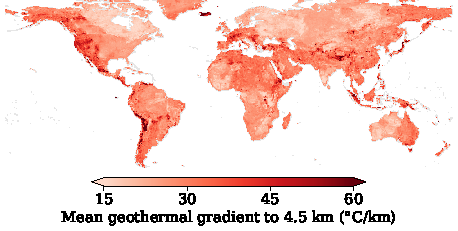
\includegraphics[width=\linewidth]{../../../misc-quarter1/geothermal/figures/egs_doc_gradient.pdf}
\caption{Mean geothermal gradient to 4.5~km}
\end{subfigure}\hfill
\begin{subfigure}[t]{0.49\textwidth}\centering
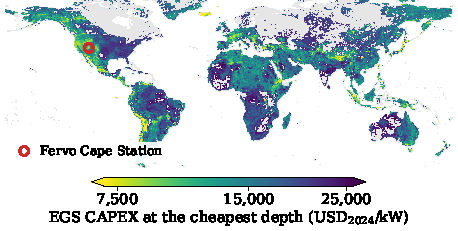
\includegraphics[width=\linewidth]{../../../misc-quarter1/geothermal/figures/egs_doc_capex.pdf}
\caption{EGS CAPEX at the cheapest depth}
\end{subfigure}
\caption{
  Enhanced geothermal on land, 0.25$^\circ$ cells.
  Left: mean temperature gradient from the surface to 4.5~km, from heat conduction on the heat-flow map of \citet{lucazeau2019}.
  Right: CAPEX per kW of net output at each cell's cheapest depth from the cost model of \citet{ricks2025}, 2025 baseline without learning; grey: no reservoir of at least 150\,\textdegree C down to 6.5~km.
  Red circle: Fervo Cape Station, the reference site of Table~\ref{tab:costs} and Figure~\ref{fig:egs}.
  CAPEX colour scale logarithmic.
}
\label{fig:egs-maps}
\end{figure}

\begin{figure}[htbp]\centering
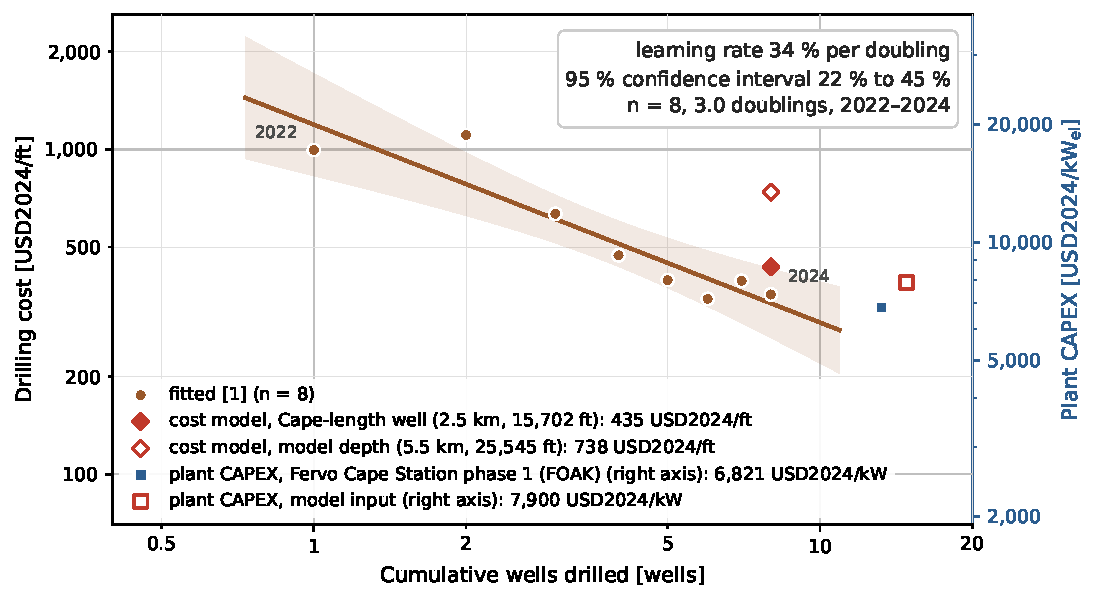
\includegraphics[width=\textwidth]{../../../misc-quarter1/technology-costs/figures/learning/egs.pdf}
\caption{Fervo Cape Station, Utah (red circle in Figure~\ref{fig:egs-maps}): drilling cost per foot of Fervo's EGS wells against cumulative wells drilled, and whole-plant CAPEX.
The first two wells are Fervo's Project Red in Nevada, all others are at Cape Station.
Source: [1] El-Sadi et al.\ (2024), as tabulated by \citet{akindipe2025}.
Red diamonds: the cost model of \citet{ricks2025} at the Cape Station cell, for a well of Cape's length (filled) and at the model's cheapest depth (hollow), drawn at Fervo's eighth well.
Squares, right axis: whole-plant CAPEX, Fervo's estimate for Cape Station phase~1 \citep{fervos1} (filled) and the model input of Table~\ref{tab:costs} (hollow), drawn at the right, without meaning on the $x$-axis.}\label{fig:egs}
\end{figure}

Regarding learning, we inherit the assumptions of \citet{ricks2025}, which split cost reductions into the wellfield and the surface plant.
Wellfield costs (drilling and stimulation) fall by 15\,\% per doubling, starting from 500~MW of EGS assumed by 2030, and surface binary plants by 10\,\% per doubling, starting from about 4~GW of binary capacity worldwide.
We do not carry their additional R\&D-driven decline of 0.5\,\% per year.
Fervo's first eight wells show faster drilling learning of 34\,\% per doubling (Figure~\ref{fig:egs}), but over only three doublings.

The fixed O\&M of 164~\$/kW/yr is the cost model's value at Cape Station, and the lifetime is 30~years.
The capacity factor of 0.85 lies between the 0.8 that NREL's ATB uses for binary plants and 0.9 \citep{atb2024}.
Existing capacity is Fervo's Project Red; the pipeline is Fervo's Cape Station (500~MW by 2028).
The lead time is 3~years.

% Conventional hydrothermal geothermal is a separate, mature row (Section~\ref{sec:geothermal}).
